% CHAPITRE 4
\chapter{Effets de l'hydrologie sur les flux de CO2 et CH4}

\minitoc

\newpage

%\section{Manipulation du niveau de l'eau en mésocosmes}
\section{Introduction}

Au cours des deux années qu'ont durées des suivis des émissions de flux de \coo et de \chh sur la tourbière de La Guette, le niveau de la nappe n'a que très faiblement varié par rapport aux années précédentes bien plus sèches.
De cette faible ou absente variation a résulté du faible lien entre le niveau de la nappe et les flux de GES.
Malgré tout il est connu que ce facteur est un facteur contrôlant important des flux.

Ainsi de nombreuses études on reliées les émissions de \coo au niveau de la nappe avec, cependant, des résultats et des conclusions variables.
La majorité des études montrent qu'une tourbière dont le niveau de la nappe est abaissé, soit par un drainage, soit par une sécheresse, aura tendance à avoir un ENE plus faible :
Ainsi \citet{strack2013} expliquent des valeurs d'ENE plus faibles qu'escompté, par des mesures faites pendant une période relativement sèche.
Une observation similaire est faite par \citet{aurela2007} qui mesure un ENE plus faible lors d'une année sèche, sur une tourbière à Carex du sud de la Finlande.
Ils attribuent la variation de l'ENE à une augmentation de la RE et à une baisse de la PPB, dans des conditions plus chaudes et plus sèches.
\citet{peichl2014} observent également une baisse de l'ENE lors d'une année ou le niveau de la nappe baisse de façon importante, au de-là de \SI{-30}{\centi\metre}.
Ils expliquent cette baisse par une baisse de la PPB qui serait liée principalement à un effet de seuil présent à \SI{-30}{\centi\metre}.
À cette profondeur se situerait la limite de la sphère racinaire et la limite au delà de laquelle les forces capillaires ne sont plus assez forte pour maintenir un approvisionnement en eau suffisant pour les sphaignes.
Cette observation va dans le même sens que \citet{lund2012} qui attribuent également à une baisse de la PPB la baisse de l'ENE qu'ils observent en 2008 sur une tourbière située au sud de la Suède, les mesures de RE étant cette année là similaires à celles observées les autres années de mesure.
Mais dans cette même étude, pour la même tourbière, \citet{lund2012} expliquent une baisse de l'ENE, en 2006 cette fois, par une augmentation de la RE, tandis que cette année au contraire les flux de PPB sont ceux qui sont similaires à ceux des autres années.
Ce paradoxe apparent est interprété grâce au type de sécheresse : courte et intense pendant la saison de végétation de 2006 et d'intensité plus faible mais d'une durée plus longue en 2008.
Enfin et à l'inverse des résultats précédemment cités, \citet{ballantyne2014} dans une étude des effets à long terme d'une baisse du niveau de la nappe, n'observe que peu d'effet sur l'ENE tandis que les flux de RE et de PPB augmentent tous deux.
Toutes ces études montrent que si le niveau de la nappe est incontestablement reconnu comme un facteur de contrôle des flux de \coo, il est difficile d'en dégager, avec certitude, un comportement valable de façon générale.
Concernant le méthane, une baisse du niveau de la nappe est généralement liée à une baisse des émissions de \chh, et inversement \citep{strack2006,pelletier2007,turetsky2008}.
Cependant d'autres études, principalement dans des sites ou le niveau de la nappe est proche de la surface du sol, montrent une absence de relation entre le niveau de la nappe et les émissions de méthane, voire une relation inverse, avec des flux plus faibles liés à des niveaux de nappe plus élevés \citep{kettunen1996,bellisario1999,treat2007}.
Là encore selon les conditions environnementales, la relation entre les flux de \chh et le niveau de la nappe n'est pas généralisable.

L'objectif de ce chapitre est donc d'explorer plus en avant l'effet du niveau de la nappe sur les émissions de GES, effet peu ou pas visible \textit{in-situ}.
Plus précisément il s'agit de déterminer l'effet de cycles de dessication/ré-humectation sur les émissions de \coo et de \chh. 
%\citet{treat2007} montre également que selon l'échelle de temps le niveau de la nappe peut être corrélé soit négativement, soit positivement avec les flux de \chh.

\section{Procédure expérimentale}

L'étude des cycles de dessication/ré-humectation s'est effectué sur des mésocosmes, prélevés sur la tourbière de La Guette.
L'expérimentation a été testé durant l'été 2013 avec un seul cycle, on s'y référera par la suite comme l'expérimentation A.
Cette expérimentation a été renouvelée l'été 2014 afin d'augmenter à trois le nombre de cycles, on l'appelera l'expérimentation B (Tableau~\ref{table:recap_hm}).

\subsection{Expérimentation A}
Le 12 avril 2013, ont été prélevés, sur la tourbière de La Guette 6 mésocosmes.
Le prélèvement de mésocosmes s'effectue à l'aide de cylindres de PVC qui, dans un premier temps, posé sur le sol, permettent de faire un pré-découpage au couteau, puis dans un second temps sont insérés, délicatement, dans la tourbe. 
Les mésocosmes sont finalement dégagés en creusant de chaque côté (Figure~\ref{fig:mesophoto}).
Les mésocosmes sont transportés au laboratoire ou ils sont enterrés en extérieur et saturé en eau (eau prélevée dans la tourbière).
Trois mésocosmes sont choisi pour servir de contrôle, et trois vont subir un cycle de dessication/ré-humectation.
%À partir du 31 mars 2013 de l'eau a été pompé régulièrement dans les 3 mésocosmes traités pour simuler une sécheresse, jusqu'au 17 juillet.
À partir du 31 mars 2013 les précipitations ont été interceptées à l'aide d'abri bâchés installable rapidement en cas de pluie et la nuit.
Ces interceptions ont été faites jusqu'au 17 juillet dans les 3 mésocosmes traités pour simuler une sécheresse.
À cette date de l'eau est ajouté aux mésocosmes, que ce soit les contrôles ou les traitements, pour simuler de fortes précipitations.

\subsection{Expérimentation B}
Le 17 avril 2014, 6 nouveaux mésocosmes ont été prélevés sur la tourbières de La Guette et installé près du laboratoire, en suivant le même protocole que pour l'expérimentation A.
Une station météo a été installée à côté des mésocosmes afin de mesurer la température de l'air, l'humidité relative, l'irradiation solaire, la vitesse et la direction du vent et les précipitations toutes les 15 minutes.
Cette station permettait également l'enregistrement des températures mesurées par des sondes (T107) installées à \num{-5}, \num{-10}, et \SI{-20}{\centi\metre}.
Le premier cycle de dessication/réhumectation dura du 30 juin au 6 juillet pour la phase de dessication est du 7 au 16 juillet pour la phase de réhumectation.
Le deuxième cycle dura du 17 au 28 juillet et du 29 juillet au 3 aout, 
Enfin le dernier cycle fut mesuré du 4 au 11 aout pour la dessication et du 12 au 14 aout pour la réhumectation.



\begin{figure}
\centering
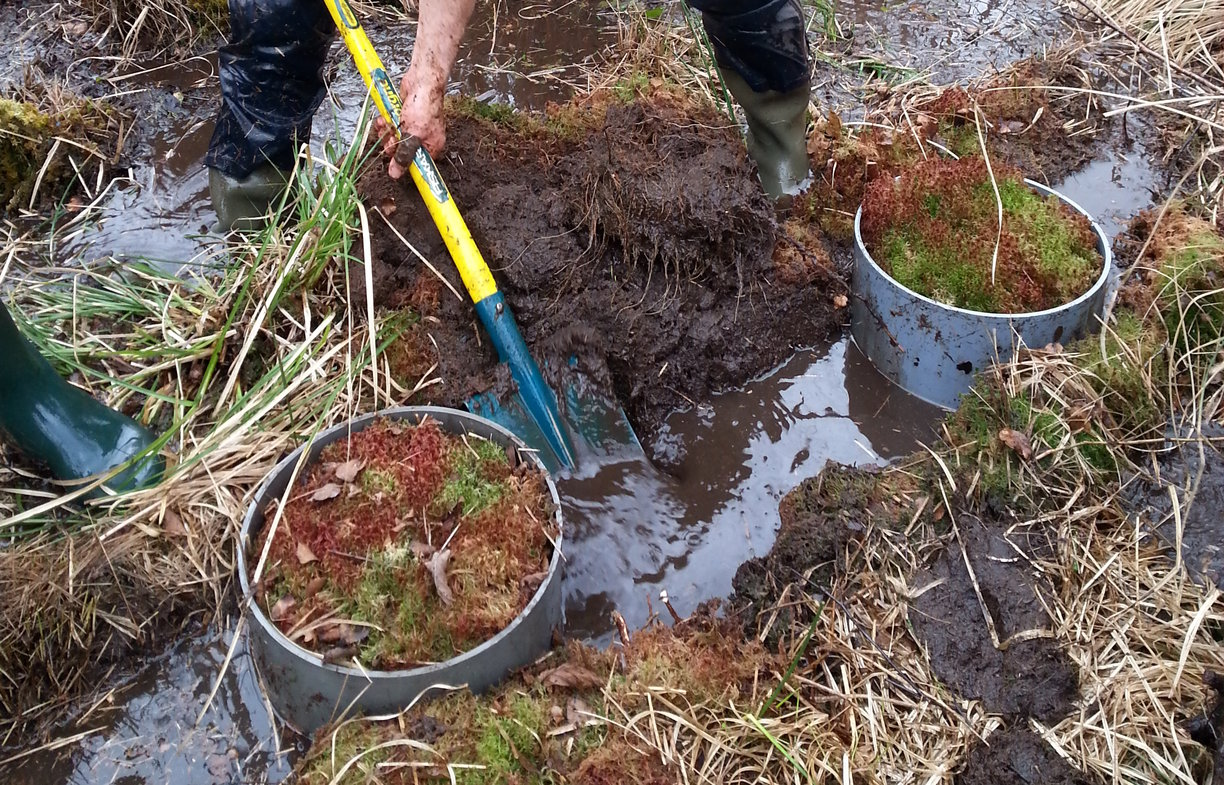
\includegraphics[width=\textwidth]{chap4/mesocosmes}
\caption{Prélèvement des mésocosmes}
\label{fig:mesophoto}
\end{figure}


\begin{table}
\centering
\caption{Récapitulatif des mesures pour les deux expérimentations}
\label{table:recap_hm}
\begin{tabular}{lll}\toprule
expérimentation & A & B \\ \midrule
année & 2013 & 2014 \\
réplicats & 6 & 6 \\
cycles & 1 & 3 \\
station météo & ? & oui\\

% & \multicolumn{2}{l}{expérimentation A} & \multicolumn{2}{l}{expérimentation B} \\ \midrule
%date &  \num{2013} & \num{1023} & \num{-308} \\
%2 &  \num{1045} & \num{1385} & \num{-340} \\
%3 &  \num{1323} & \num{1057} & \num{266} \\
%4 &  \num{1002} & \num{1262} & \num{-260} \\
\bottomrule
\end{tabular}
\end{table}


\begin{figure}
\centering
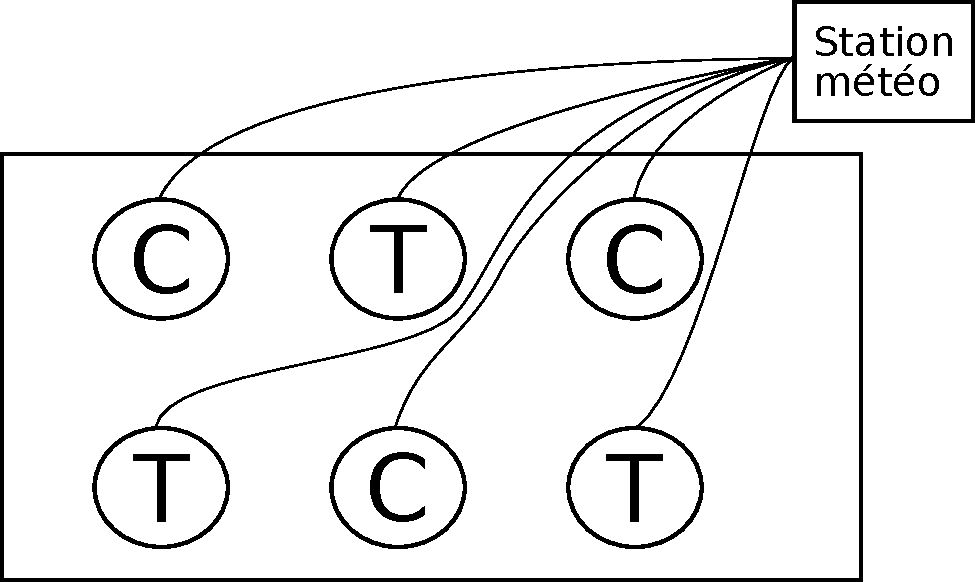
\includegraphics[width=.5\textwidth]{chap4/mesocarte}
\caption{Carte mésocosmes Zi}
\label{fig:mesocarte}
\end{figure}

%\begin{figure}
%\centering
%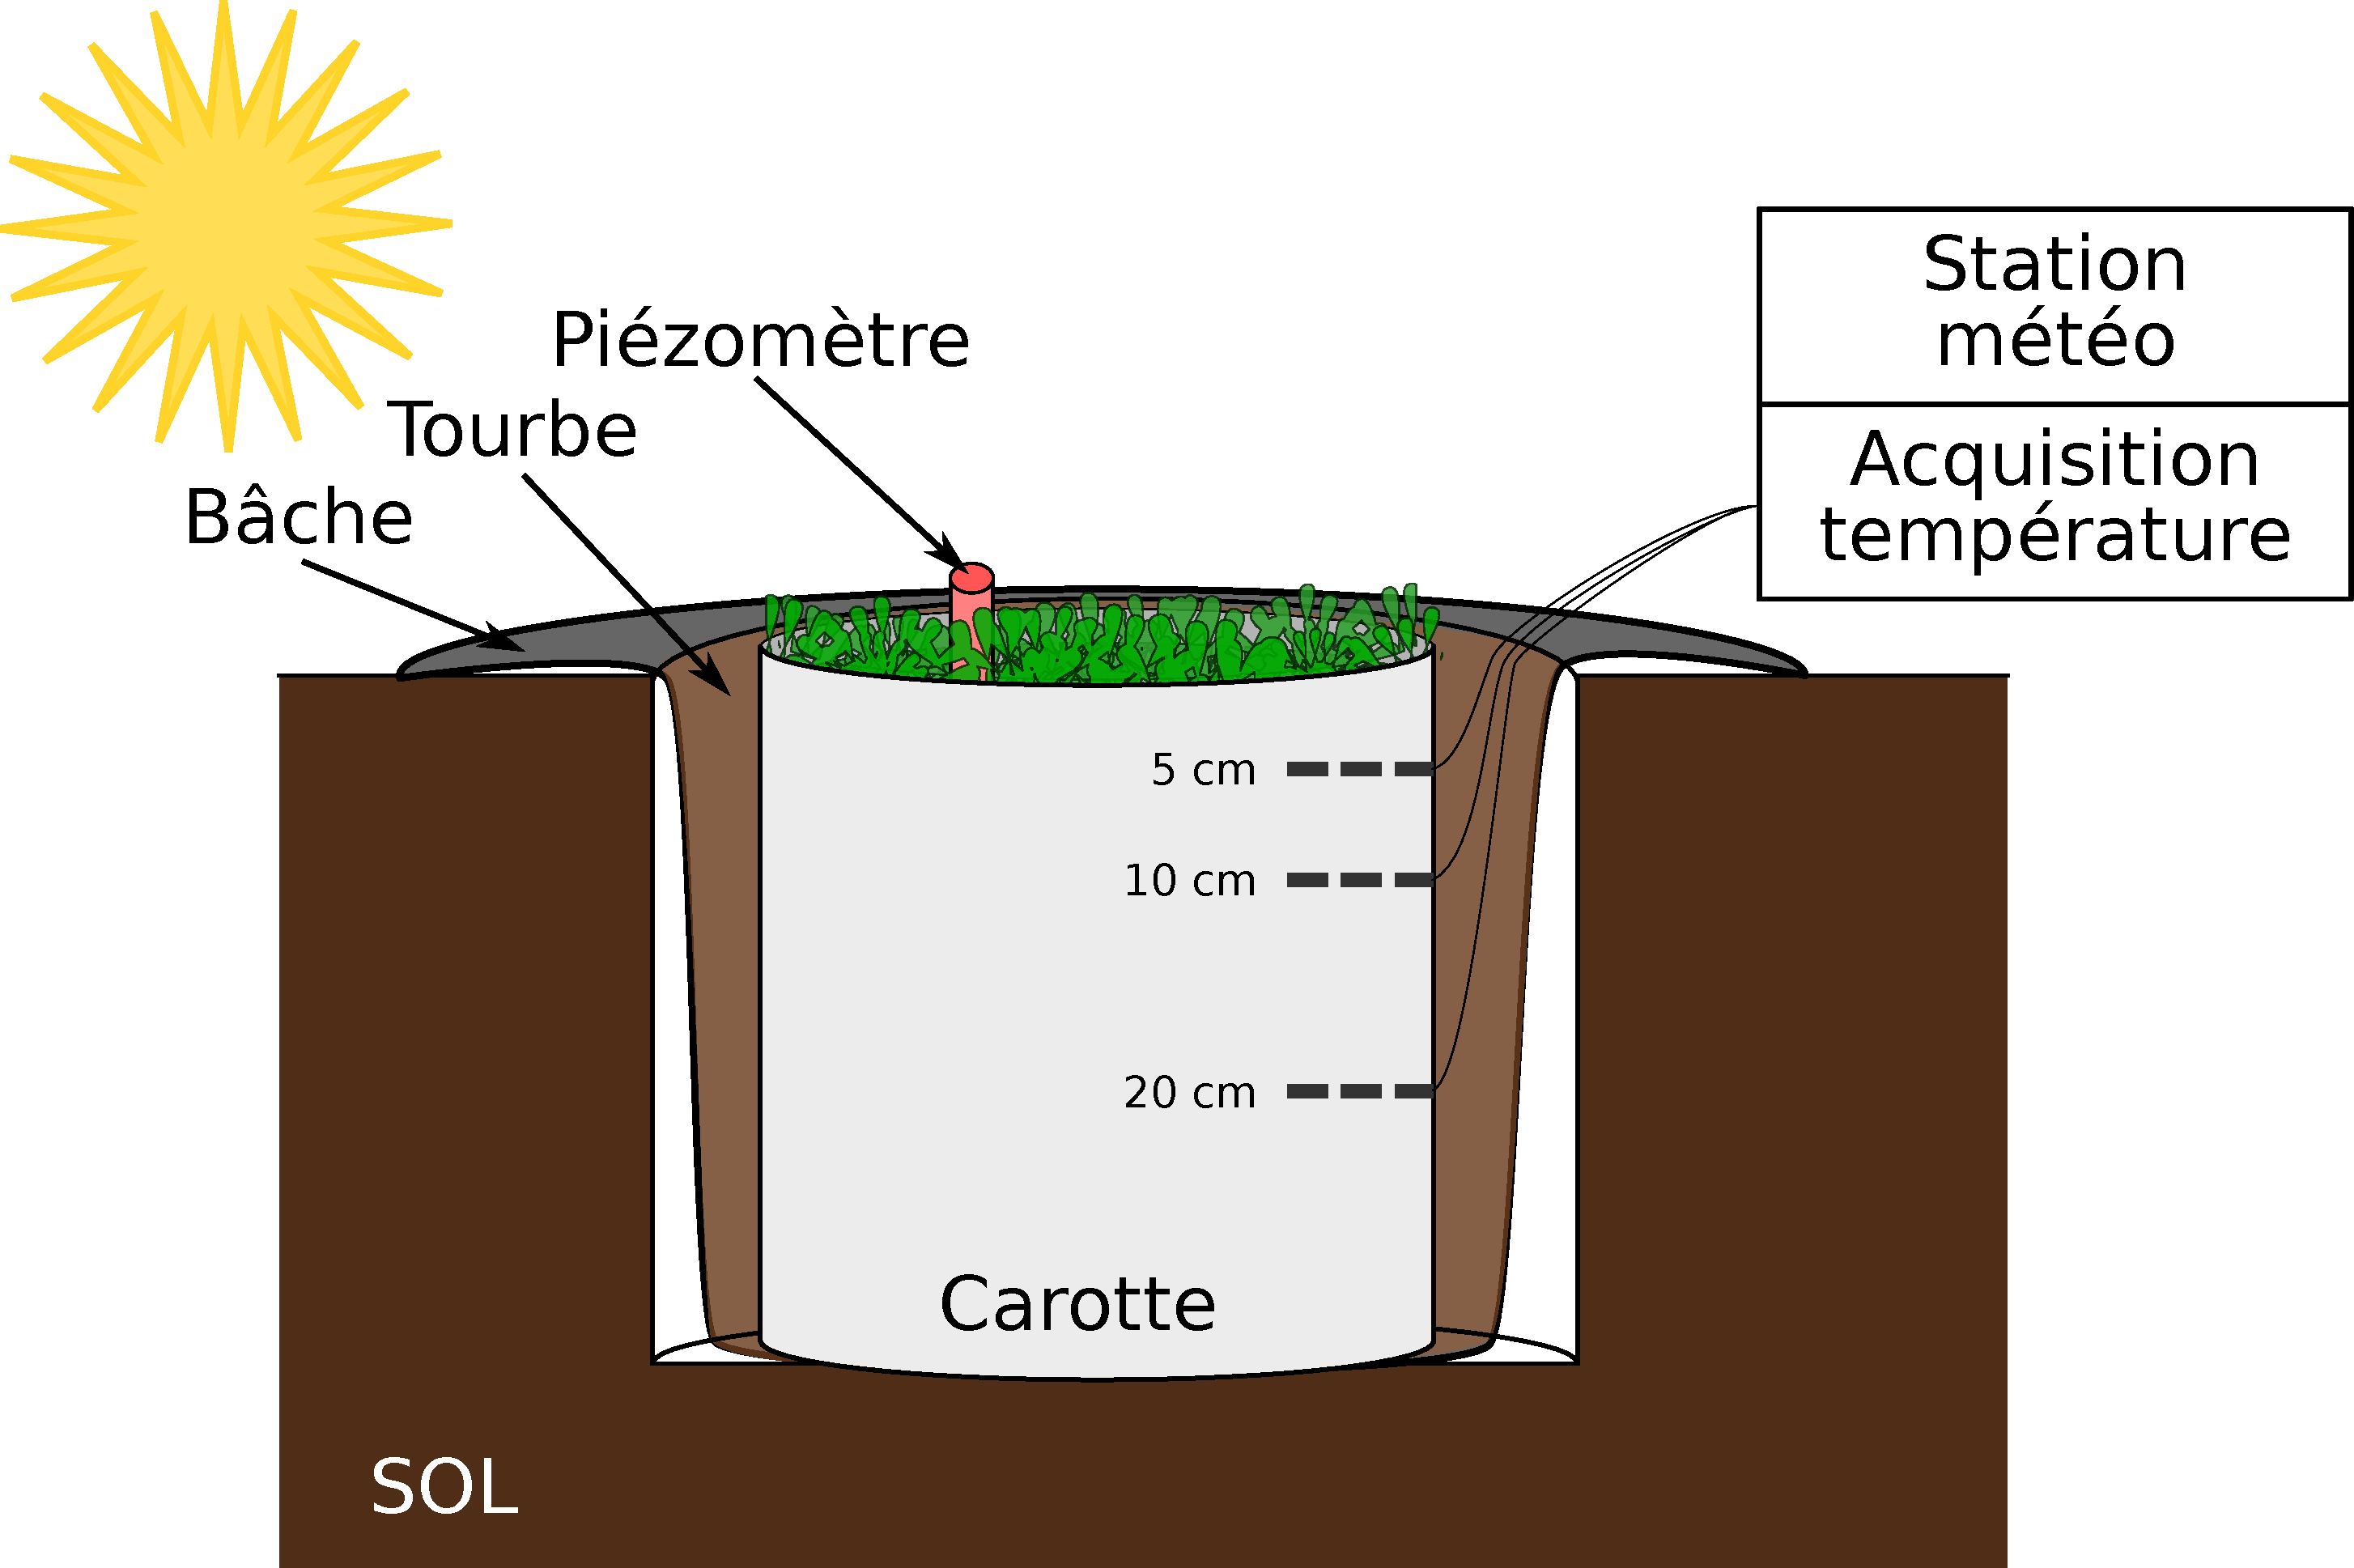
\includegraphics[width=.5\textwidth]{chap4/mesoinstall}
%\caption{Schéma d'un mésocosme}
%\label{fig:mesoinstall}
%\end{figure}

\section{Résultats}

\subsection{Expérimentation A}

Pendant la phase de dessication de l'expérimentation A, on observe une baisse du niveau de la nappe pour les placettes contrôles comme pour les placettes traitements.
Malgré tout leur comportement est différent : les placettes contrôles ont un niveau de nappe relativement élevé jusqu'au 24 juin puis ce niveau baisse fortement alors que les placettes du groupe traité ont un niveau de nappe qui diminue de façon plus continue sur l'ensemble de la phase.
La remontée du niveau de la nappe s'effectue de façon similaire pour les deux groupes.
Enfin après la phase de ré-humectation, le niveau de la nappe baisse à nouveau, plus rapidement pour le groupe traitement que pour le groupe contrôle.


\begin{figure}
\centering
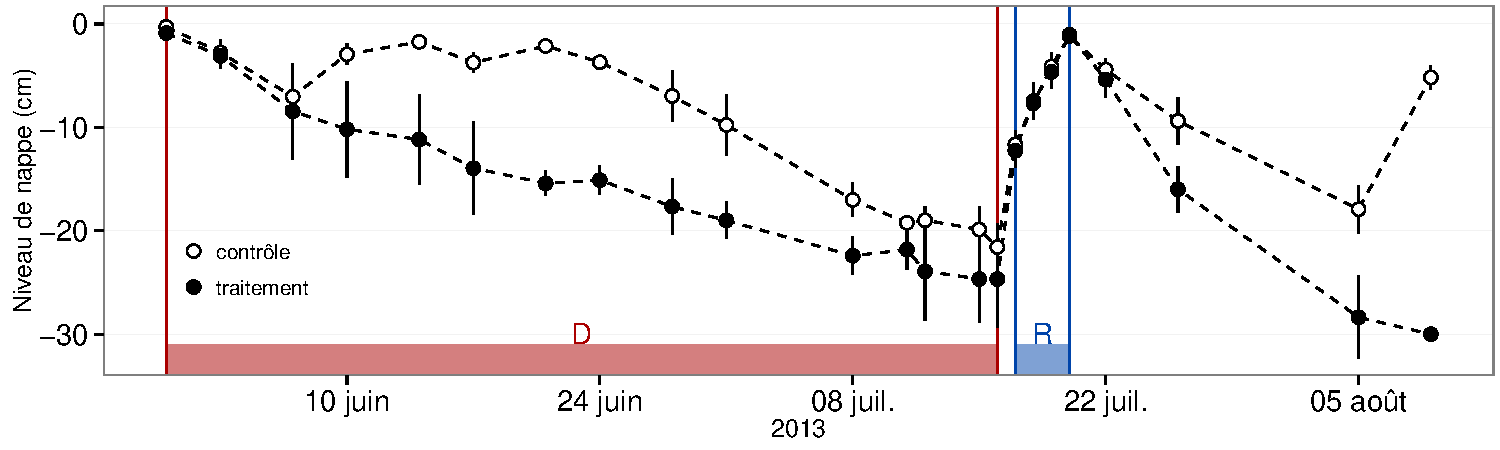
\includegraphics[width=1.15\textwidth, center]{chap4/HMzi_wtl}
\caption{Évolution du niveau de la nappe dans les mésocosmes Zi}
\label{fig:HMzi_wtl}
\end{figure}

%\begin{figure}
%\centering
%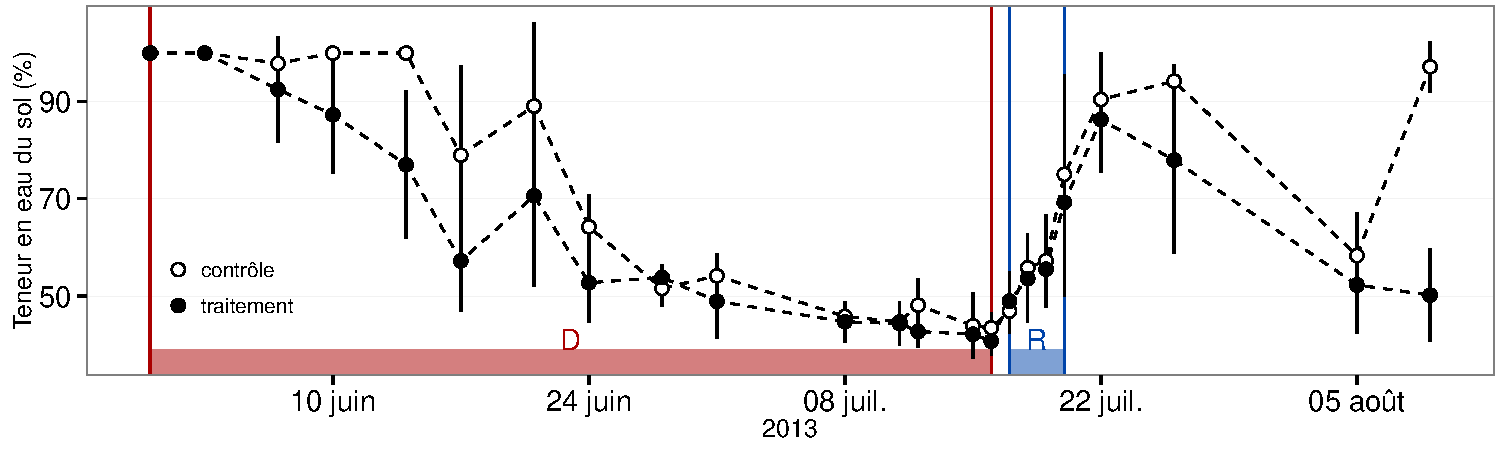
\includegraphics[width=\textwidth]{chap4/HMzi_TES}
%\caption{Évolution de la teneur en eau du sol dans les mésocosmes Zi}
%\label{fig:HMzi_TES}
%\end{figure}

\begin{figure}
\centering
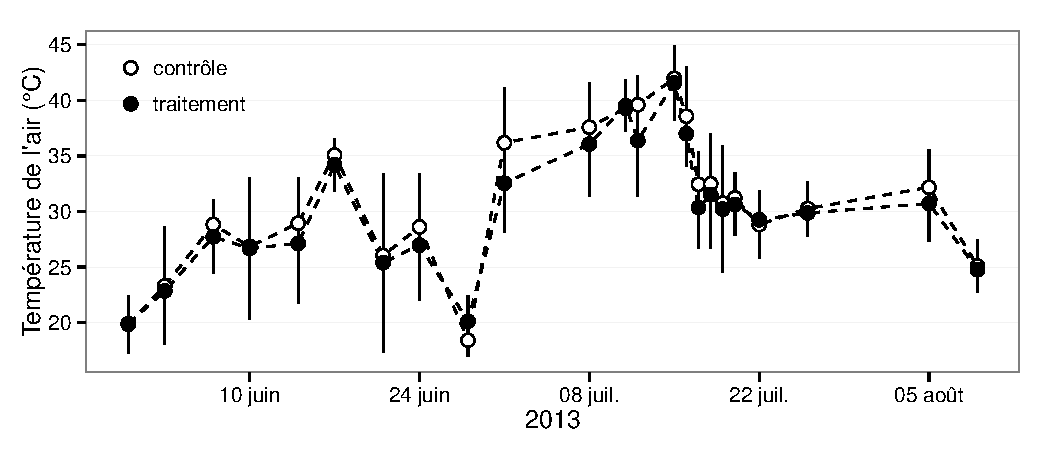
\includegraphics[width=1.15\textwidth, center]{chap4/HMzi_Tair}
\caption{Évolution de la température de l'air dans les mésocosmes Zi}
\label{fig:HMzi_Tair}
\end{figure}

Les émissions de \chh sont relativement similaires entre les deux groupes jusqu'au 24 juin 2013 (Figure~\ref{fig:HMzi_ch4}).
À cette date les émissions du groupe contrôle augmente rapidement tandis que celle des traitements reste stable.
Finalement à la fin de la phase de dessiccation les deux groupes retrouvent des niveaux d'émission similaires.
Par ailleurs ces niveaux restent constant pendant la phase de réhumectation, avant d'augmenter par la suite.
À l'exception de la forte hausse, fin juin, début juillet, du groupe contrôle, les valeurs de méthane sont comprise entre 0 et \SI{0.3}{\uml}.
Ces valeurs sont un peu plus élevée, mais du même ordre de grandeur que celles mesurées sur le terrain.

\begin{figure}
\centering
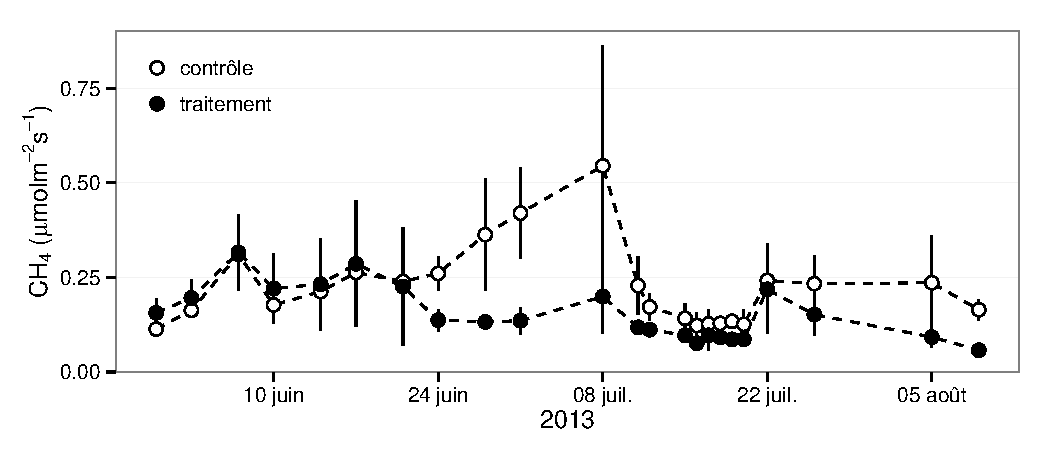
\includegraphics[width=1.15\textwidth, center]{chap4/HMzi_ch4}
\caption{Évolution du méthane dans les mésocosmes Zi}
\label{fig:HMzi_ch4}
\end{figure}

La Re du groupe traité augmente régulièrement pendant la phase de dessiccation (Figure~\ref{fig:HMty_ER}).
Le comportement du groupe de contrôle est, une fois encore, séparé en deux : relativement stable, avec des valeurs inférieures à celle du groupe traité, jusqu'à fin juin puis une augmentation importante début juillet ou la RE dépasse puis rejoint les valeurs mesurées pour le groupe contrôle.
Les deux groupes voient les valeurs de leur RE diminuer de la même façon pendant la phase de réhumectation.
Finalement, après cette phase, les valeurs de RE augmentent jusqu'à retrouver des valeurs proches de celle mesurées à la fin de la phase de dessication.
Les valeurs de RE mesurées sont dans la gamme de celles mesurées sur le terrain, avec cependant des maximums moins importants.

\begin{figure}
\centering
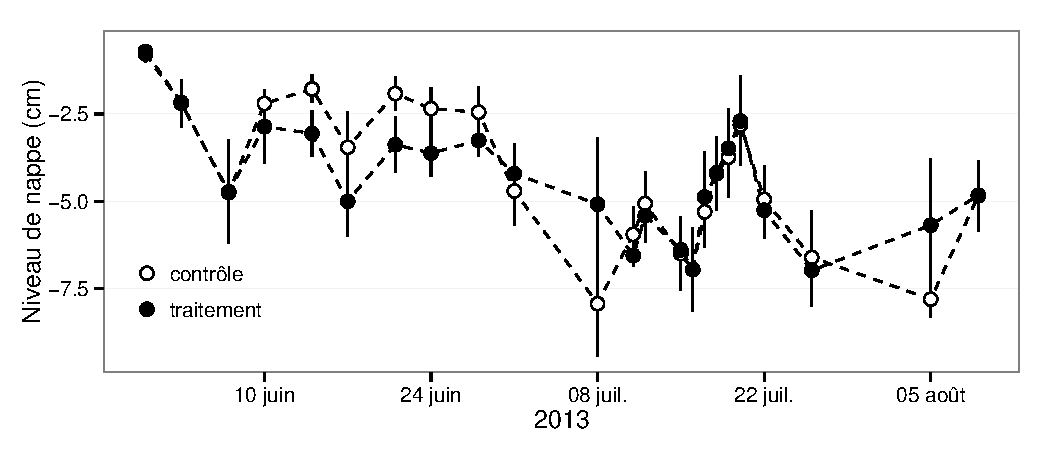
\includegraphics[width=1.15\textwidth, center]{chap4/HMzi_ER}
\caption{Évolution de la RE dans les mésocosmes Zi}
\label{fig:HMzi_ER}
\end{figure}

L'ENE mesurées sur les deux groupes est systématiquement supérieure pour le groupe contrôle, avec une évolution parallèle des flux pour les deux groupes (Figure~\ref{fig:HMzi_NEE}).
Pendant la phase de dessiccation l'ENE reste constante jusque fin juin avec un écart entre le groupe contrôle et le groupe traitement qui tend à augmenter.
Puis l'ENE diminue à partir de début juillet, les deux groupes ayant des valeurs très proches.
L'ENE augmente pendant la phase de réhumectation avant de se stabiliser par la suite.

\begin{figure}
\centering
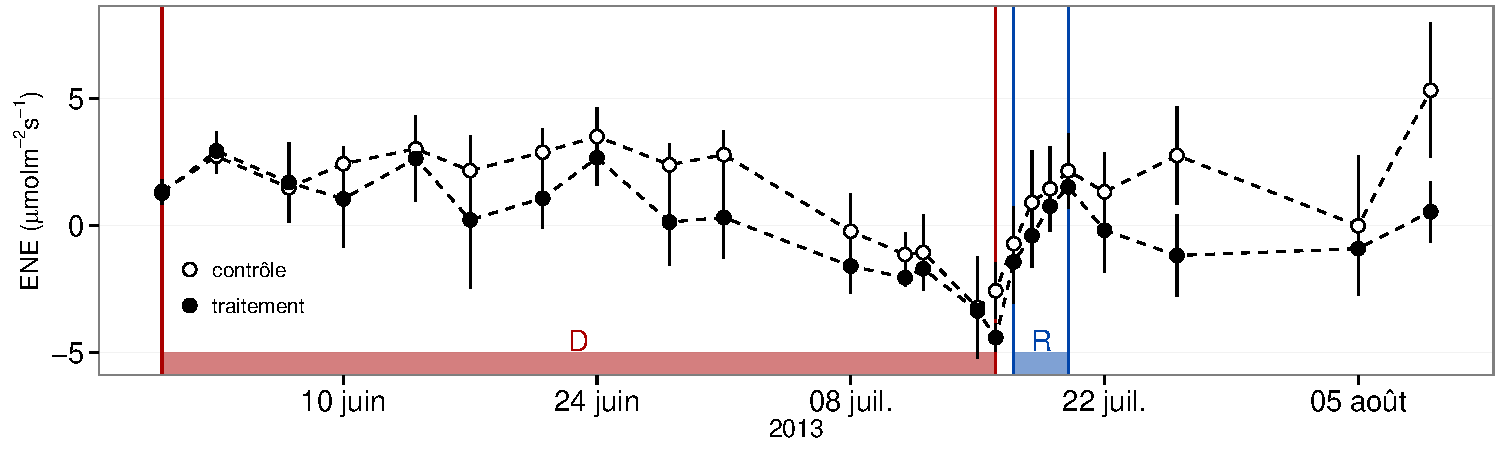
\includegraphics[width=1.15\textwidth, center]{chap4/HMzi_NEE}
\caption{Évolution de la NEE dans les mésocosmes Zi}
\label{fig:HMzi_NEE}
\end{figure}


\begin{figure}
\centering
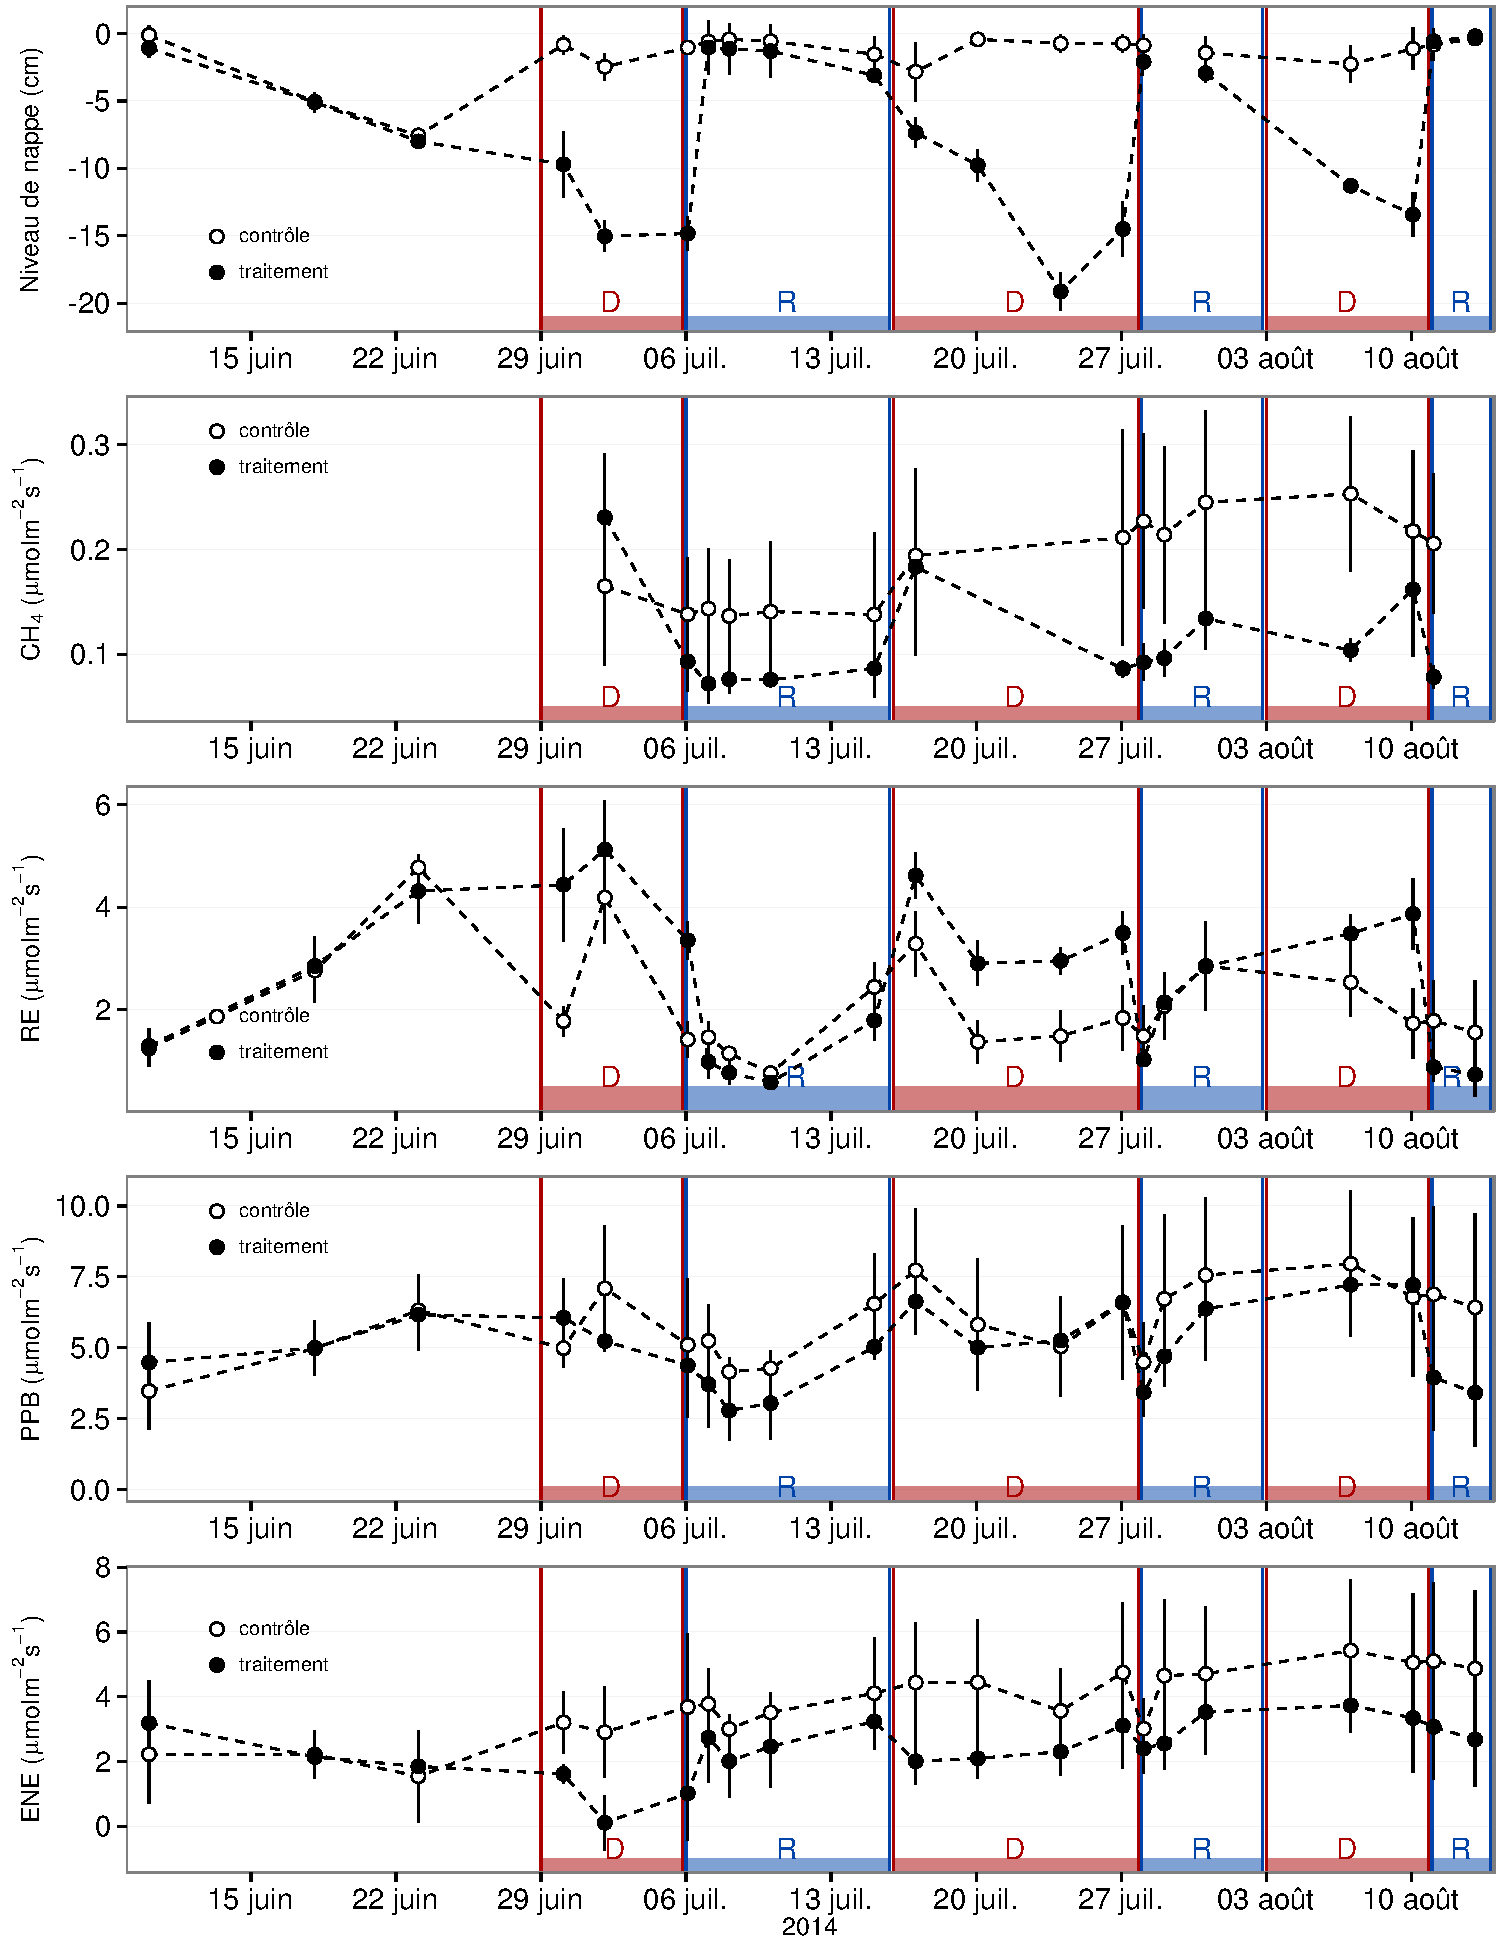
\includegraphics[width=1.15\textwidth, center]{chap4/expB_flux}
\caption{Évolution du niveau de la nappe dans les mésocosmes Tianyi}
\label{fig:HMty}
\end{figure}

\subsection{Expérimentation B}

Contrairement à l'expérimentation A, et à cause d'une météo moins ensoleillée, le niveau de nappe du groupe de contrôle de l'expérimentation B reste relativement constant pendant l'ensemble de la période de mesure (Figure~\ref{fig:HMty}--A).
Le drainage artificiel du groupe traité permet d'abaisser le niveau de la nappe d'une quinzaine de centimètres en moyenne pour chaque cycle.

Les émissions de \chh mesuré lors de l'expérimentation B sont du même ordre de grandeur, entre 0 et \SI{0.3}{\uml}, que celles mesurées \textit{in-situ}, sur la tourbière de La Guette (Figure~\ref{fig:HMty}--B).
À l'exception du point mesuré lors de la première phase de dessiccation, les valeurs du groupe de contrôle sont systématiquement supérieures à celles du groupe traité.
Les émissions du groupe de contrôle tendent à augmenter sur la période de mesure.
Cette tendance est également visible pour le groupe traité.
Concernant les cycles de dessiccation/réhumectation, il est difficile de dégager des comportements communs, même s'il semble que l'assèchement conduit à une baisse des émissions.
Un pic d'émission de \chh est également à noter pour chaque cycle pendant la phase de dessiccation.

Les valeurs RE mesurées sur les mésocomes sont plus faible que celle relevées directement sur la tourbière de La Guette avec un maximum moyen à 5 contre \SI{8}{\uml} mesuré sur le site.
Avant le début des traitement d'assèchement, les flux de la RE sont proches pour les deux groupes tandis qu'après, leurs comportements diffèrent (Figure~\ref{fig:HMty}--C)).
Pendant les phases de dessiccation la RE du groupe traité est supérieure à celle du groupe de contrôle.
La relation semble s'inverser pendant les phases de réhumectation, du moins pour les cycles 1 et 3, car pendant la phase de réhumectation du cycle 2 les deux groupes ont des valeurs similaires.


Comme pour la RE, les flux de PPB sont du même ordre de grandeur que ceux mesurés sur le terrain, mais légèrement plus faible : les maximas moyens mesurés dans les mésocosmes sont d'environ \num{7.5} pour des valeurs de \SI{13}{\uml} mesuré directement sur la tourbière (Figure~\ref{fig:HMty}--D).
Avant le début des traitements les flux des deux groupes sont similaires.
La première phase de dessiccation fait passer la PPB du groupe de contrôle au dessus du groupe traité.
Pour les deux groupes, la PPB est plus importante lors des phases de dessiccation comparée aux phase de réhumectation, avec des moyennes respectives de \num{6.35(219)} contre \num{5.80(220)} pour le groupe de contrôle et de \num{5.95(146)} contre \SI{4.05(160)}{\uml} pour le groupe traité.

Les flux de l'ENE sont similaires pour les deux groupes avant le début du traitement (Figure~\ref{fig:HMty}--E).
Le premier cycle de dessiccation/réhumectation divise les deux groupes : le groupe de contrôle ayant des valeurs d'ENE plus élevées que celles du groupe traité.
L'évolution des deux groupes reste cependant relativement conjointe pendant la période de mesure avec une tendance à la hausse.

%\begin{figure}
%\centering
%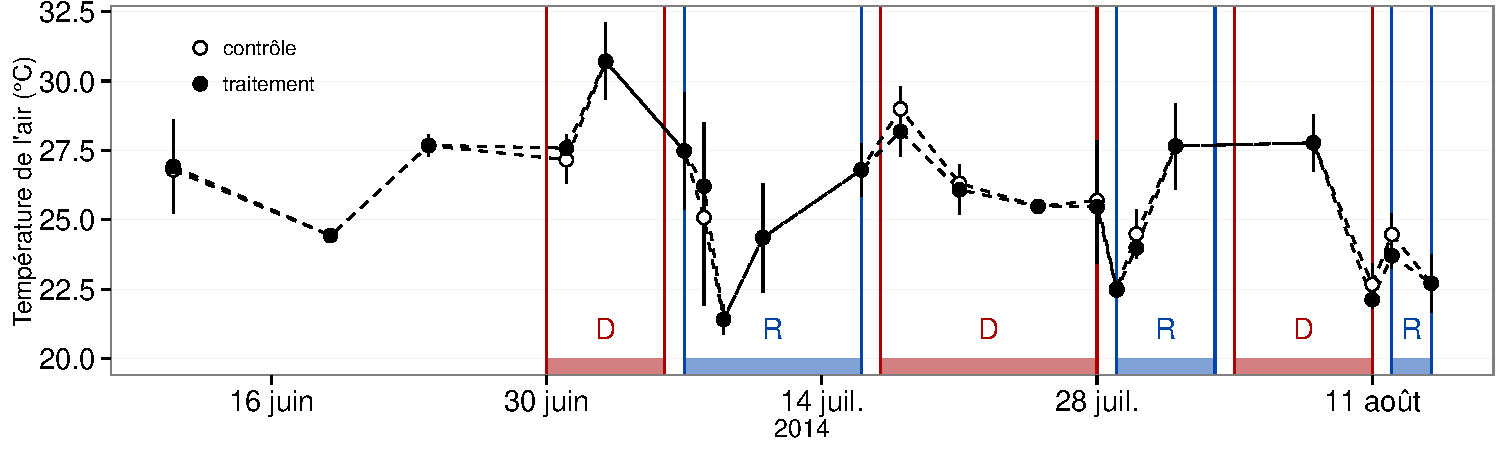
\includegraphics[width=1.15\textwidth, center]{chap4/HMty_Tair}
%\caption{Évolution du niveau de la nappe dans les mésocosmes Tianyi}
%\label{fig:HMty_tair}
%\end{figure}
%
%\begin{figure}
%\centering
%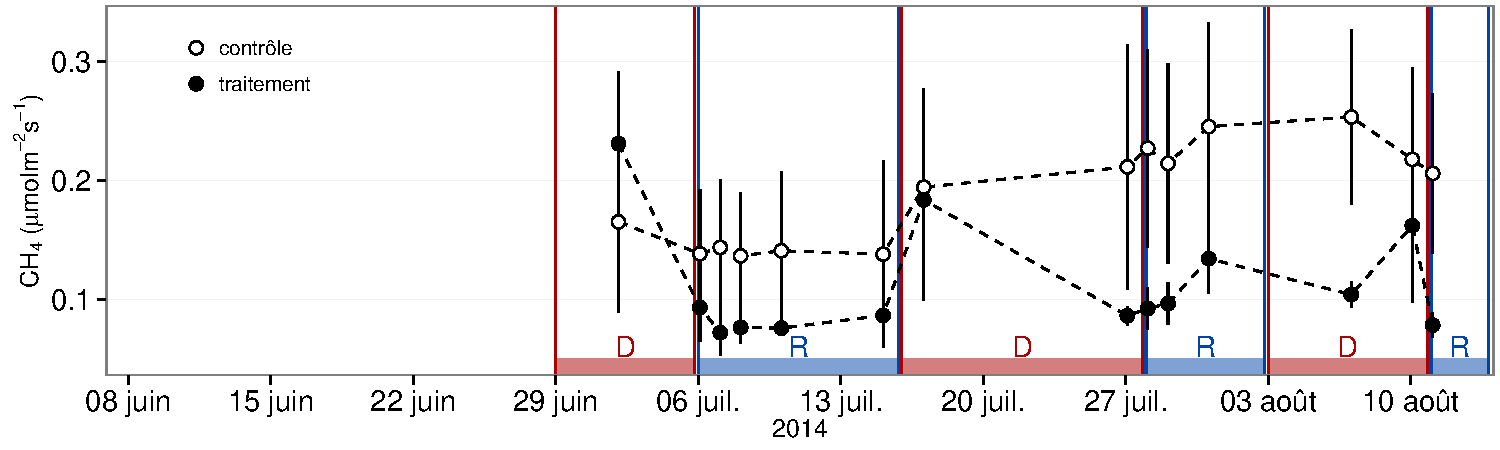
\includegraphics[width=1.15\textwidth, center]{chap4/HMty_ch4}
%\caption{Évolution du niveau de la nappe dans les mésocosmes Tianyi}
%\label{fig:HMty_ch4}
%\end{figure}
%
%\begin{figure}
%\centering
%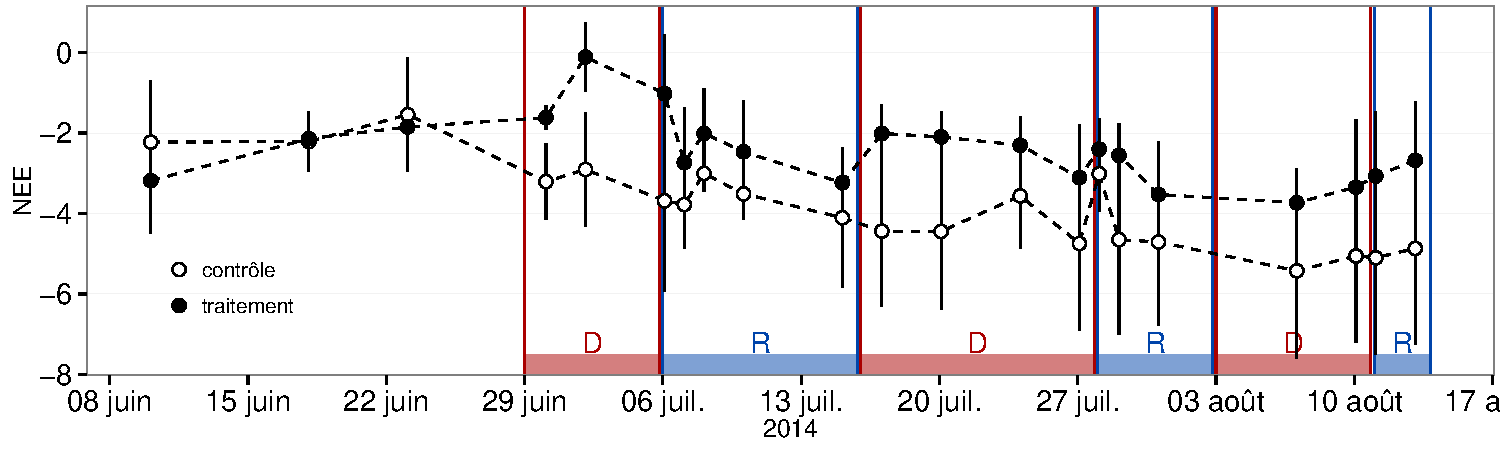
\includegraphics[width=1.15\textwidth, center]{chap4/HMty_NEE}
%\caption{Évolution de la NEE dans les mésocosmes Tianyi}
%\label{fig:HMty_NEE}
%\end{figure}
%
%\begin{figure}
%\centering
%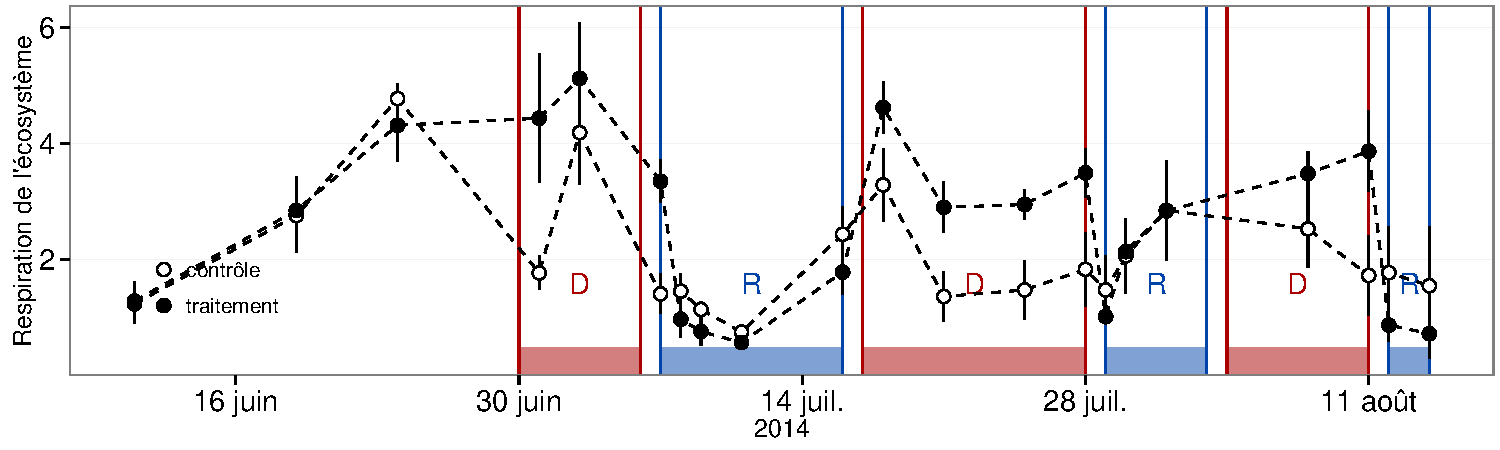
\includegraphics[width=1.15\textwidth, center]{chap4/HMty_ER}
%\caption{Évolution de la RE dans les mésocosmes Tianyi}
%\label{fig:HMty_ER}
%\end{figure}

\subsection{Dessication}

\begin{itemize}
\item augmentation RE
\item diminution CH4
\end{itemize}

\subsection{Événement pluvieux}

\begin{itemize}
\item diminution RE
\item augmentation CH4 avec retard
\end{itemize}

\subsection{Effet cycles multiples}

\section{Discussion}

%\section{Manipulation du niveau de l'eau (teneur en eau) in-situ}
%\subsection{introduction}
%L'étude des effets de l'hydrologie sur les émissions de flux de GES a également pu être menée directement in-situ au sein du projet CARBIODIV (Restauration hydrologique de la tourbière de La Guette : effets sur l'évolution de la biodiversité et le stockage du carbone.) dont l'objectif est de restaurer le fonctionnement hydrologique de la tourbière de La Guette.
%\subsection{Procédure expérimentale}
%\subsubsection{Les travaux}
%\subsubsection{Les stations scientifiques}
%Deux stations ont été installées sur le site, dans deux sous-hydrosystèmes différents. Le premier en amont n'étant pas impacté par les travaux permet de contrôler les effets de site, et le second, en aval, enregistrera les effets de la restauration hydrologique.
%\subsection{Résultats}
%\subsection{Discussion}
